In this section we present our approach to collect various website information,in order to evaluate our methodology.In order to achieve our goal ,we crawl a list of websites and analysis those data. This chapter explains the overview of those traces which we received after web crawling,data cleanup procedure and the final set of data after the clustering algorithm described in chapter-3 methodology section.
\subsection{Host name Selection}
To obtain a good coverage of the largest hosting infrastructures,
we crawl top 100,000 ranked websites from Alexa [26].Alexa ranks websites based on Internet traffic-users of its tool bar for various web browsers like Google Chrome,Internet explorer,Firefox.After crawling we are able to generate 13919464 traces.

Moreover,websites contain a lot of embedded contents like images,videos, advertisements etc. that the browser of the user has to download from the various web servers.These web servers can be from different web content providers or from  hyper giants. In our study, such embedded content has to be taken into account, as it might be served from servers other than those serving the front page of a popular host name listed in top rank websites of Alexa.To give better understanding,while crawling facebook.com,the front page is served from Facebook data centers while the logo and other meta data come from Akamai.For most of the websites,the important videos,images or other embedded contents present in the front page of the websites.So to make our study more precise,we crawl only the front pages of all the top ranked websites and the embedded links present in the front pages of those websites.

\subsection{Data Cleanup}
We perform a thorough cleanup process on the raw traces.In each crawling we gather 15 different metrics.Hence we pass each crawled link into regular expression to check the validity of the links based on number of metrics,type of matrices.

First we collect top 100,000 top ranked websites as of September 2016 from Alexa website.The scrapy crawler queries the HTTP get method to local DNS resolver for all the websites and store the results in a trace file.Each trace contain total 15 different data which are described below.
\begin{enumerate}
   \item index :index shows the rank of the website
	\item depth\_level : 0 or 1.
			  0 shows that the website is the main page url and 1 shows the embedded links inside main page 
\item httpResponseStatus :the HTTP return status code.
\item MIMEcontentType :this is included to know the type of element inside the web page.
\item content\_length :content length gives the idea about the size of the element.
\item url :this is the url to be crawled by the scrapy engine.This url can be main page url or embeded links.Duplicate links are omitted for the same main page by using RFPDupeFilter.RFPDupeFilter is a scrapy  class which is used to detect and filter duplicate requests [3].
\item cookies :cookies involved in a website
\item tagType :this shows the HTML element type.
		for example if an element is embeded in a wensite like "<img class="desktop" title="" alt="" src="img/bg-cropped.jpg">",then we collect the tagtype which is img here. 
ARecord=This contain all the aRecord names involved in a website while resolving to the ip address..
\begin{figure}[h]
\includegraphics[width=\textwidth,height=10cm]{/home/sakib/soumya/wholeSLD/dnsBmw.png}
\centering
\caption{dig for bmw.com}
\end{figure}
for the the website "www.bmw.com",the ARecord name are a1586.b.akamai.net. and a1586.b.akamai.net. which will be stored in trace will under ARecord column.
\item destIP :this column stores the corresponding resolved ip addresses of the website.For example,for the website bmw.com (figure-6),the destIP will store 72.247.184.130 and 72.247.184.137
\item ASN\_Number=Field():This column stores the ASN number of a IP address.For this we use maxmind IP to ASN mapping file.
\item distinctASNs=This will keep the total number of ASNs involved for all the embedded website links for a particular main page url which is one of the Alexa's top ranked website.
\item ObjectCount=Field():This column stores the total number of external links embedded in a website.
\item NumberOfuniqueExternalSecondlevelSites :This columns gives the total number of unique second level domains involved in all the embedded links of a website.
    \item start\_time :This contains the staring time when the HTTP starts requesting for the website.
    \item end\_time=This contains the staring time when the HTTP ends requesting for the website.
    \end{enumerate}

Through scrapy we crawled total total 13919464 website links.After data cleanup, we have 13919464 clean traces that form the basis of this study.

\subsection{Clustering Algorithm}
Overall we get total 219604 unique second level domains.But from them a lot of SLDs which can be clustered into other SLDs.After clustering algorithm we are able to get 53852 unique clustered SLD infrastructures.

\begin{figure}[h]
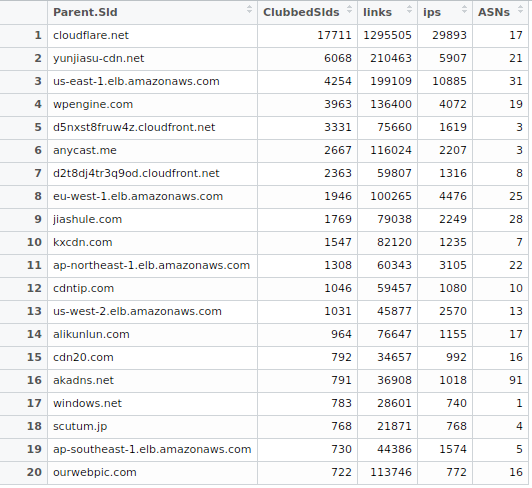
\includegraphics[width=\textwidth,height=10cm]{/home/sakib/soumya/latexNew/clubbedSlds.png}
\centering
\caption{Top 20 clustered SLD infrastructure in decreasing order of clubbed SLD count.}
\end{figure}

The top 20 clustered SLD infrastructures in the decreasing order of clubbed SLDs are shown in figure 10.The third column contain number of links served by a whole clustered SLD infrastructure.Similarly fourth column shows number of IP addresses resolved and fifth column shows the number of ASNs managed as a whole clustered SLD infrastructure.From figure we can see that under cloudflare.net,17711 number of SLDs clubbed which is  10,68 \% of all child slds clubbed.From the table also we can see three different Clustered SLD infrastructure where the main SLD having cloud flare in SLD naming pattern. cloudflare.net,d2t8dj4tr3q9od.cloudfront.net,d5nxst8fruw4z.cloudfront.net
All the three SLD infrastructures are from same parent company cloudflare.net.But they shows different clustered infrastructure which shows that they have different infrastructure from each other in terms of bgp prefixes.Similarly we can five different clustered SLD infrastructure having amazon in their SLD naming pattern.Both amazon and cloudflare are big CDNs ,they also provide a lot of other services like  Internet Security services,distributed domain name server services, web hosting service etc.Similarly amazon provide cloud computing services,infrastructure services etc. to their customers.This unveils that big hosting infrastructures maintain different SLD infrastructures separately which might they use for different purposes. 

\subsection{Web objects}
We also collected different web objects embedded in home pages of 100,000 top ranked web sites of Alexa.After crawling we found total 285 different types of objects from 219604 unique second level domains.The main web objects which shown are text/html which is around 38\% of all object types crawled.Similarly SLDs serve almost 42 \% of image files.Here it is important to notice that we only get the type of object by collecting content type header field.

\subsection{Conclusion}
In this section we define our approach of selecting SLDs after clustering algorithm.This will help to find out prominent infrastructures present in today' Internet.We also talk about different metrics considered while crawling web site.